\documentclass[slides]{pgnotes}

\title{Infrastructure}

\begin{document}

\maketitle

\tableofcontents

\section{Infrastructure requirements}

\begin{redbox}{Important reminder!}
  \begin{itemize}
  \item This section is very much an introductory tour of issues to consider when provisioning infrastructure and software to support our data architecture.
  \item Many of the themes covered here would warrant an entire 12-week module for themselves!
  \item Basic awareness avoids costly pitfalls.
  \end{itemize}
\end{redbox}

\section{Server hardware}

\begin{center}
  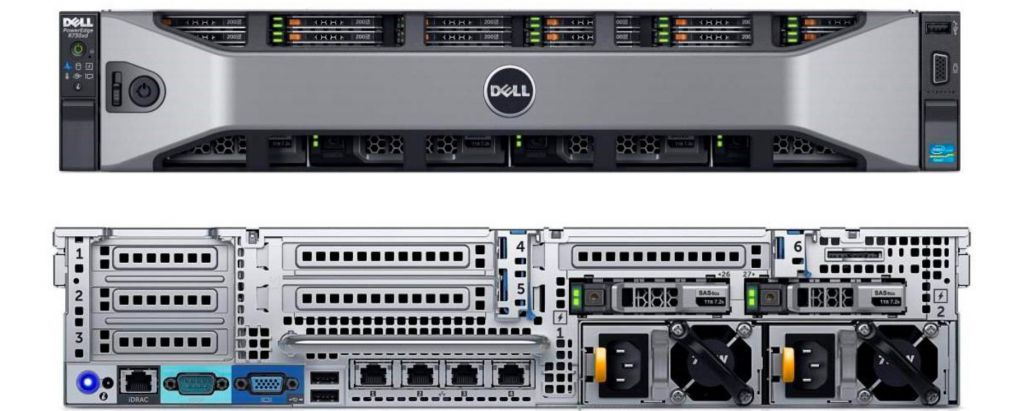
\includegraphics[width=0.8\linewidth]{dell_poweredge}
\end{center}

\subsection{Operating system}

Will need to decide what OS the server is to run.

Linux and UNIX are generally good choices for data-intensive workloads.

\begin{bluebox}{Considerations}
  \begin{itemize}
  \item Standard choice for MySQL, PostgreSQL, Oracle, MongoDB, others.
  \item Straightforward remote access (SSH)
  \end{itemize}
  \tcblower
  \begin{itemize}
  \item Different to developer environment (usually Windows)
  \end{itemize}
\end{bluebox}

Windows OS more suited for .net and/or MS SQL Server workloads.

\subsection{Specifications}

Specify based on expected workload:

\begin{bluebox}{Components}
\begin{description}

\item[CPU] based on CPU utilisation using \texttt{top, htop}.

\item[RAM] based on RAM utilisation under expected load:
  \begin{itemize}
  \item Use \texttt{free -mh}
  \end{itemize}

\item[Disk space] based on disk utilisation (projected or actual):
  \begin{itemize}
  \item Use \texttt{df -h} for system disk usage
  \item Single database:\\\texttt{SELECT pg\_size\_pretty(pg\_database\_size('Database Name'));}
  \item Interactive for all databases: \texttt{\textbackslash l+}
  \end{itemize}

\end{description}  
\end{bluebox}


\subsection{RAID}

\textbf{Redundant Array of Inexpensive Disks (RAID)} uses a number of disks in a raid set such that loss of one (or sometimes more) disks will not cause data loss.

RAID can be done in the operating system software or in hardware.



\subsubsection{RAID-1 (Mirror)}

RAID-1 duplicates information on usually 2 disks.

\begin{center}
  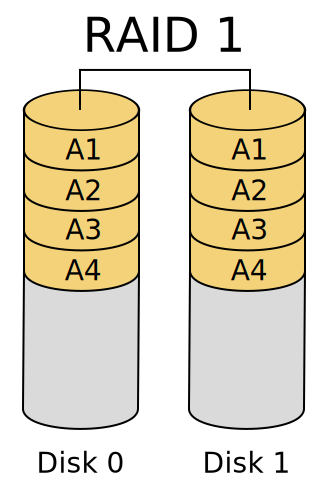
\includegraphics[width=0.2\linewidth]{raid_1}
\end{center}

Can tolerate failure and replacement of either disk without data loss.

\subsubsection{RAID-5}

RAID-5 stripes data and redundant \textit{parity} information across 3 or more disks.

\begin{center}
  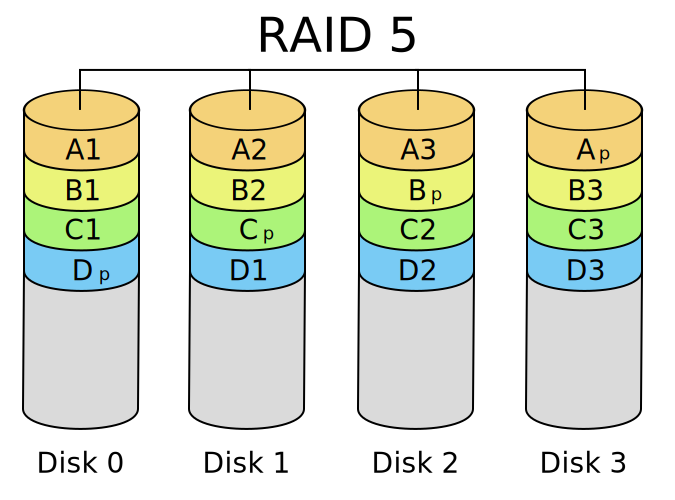
\includegraphics[width=0.4\linewidth]{raid_5}
\end{center}

Can tolerate failure and replacement of 1 disk without data loss.

\subsubsection{RAID-6}

RAID-6 stripes data and redundant \textit{parity} information across 4 or more disks.

\begin{center}
  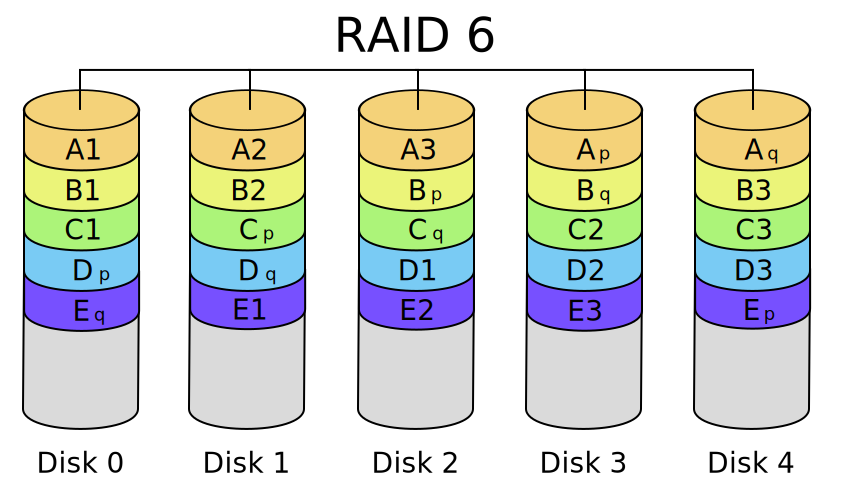
\includegraphics[width=0.4\linewidth]{raid_6}
\end{center}

Can tolerate failure and replacement of 2 disks without data loss.

\section{Data centre environment}

\begin{description}

\item[In office environment] such as under a desk, on a filing cabinet etc.
  
\item[On-site server room] possibly as part of larger campus:
  \begin{itemize}
  \item Varying levels of data centre infrastructure provision.
  \end{itemize}
\end{description}

\subsection{Co-location}

Co-location means that you / your employer bring your hardware to a dedicated data centre faciliity (a co-lo):

\begin{itemize}
\item Can rent individual rack space(s), full cabinet or entire suite / room.
\item Power supply may be included or separately chargeable
\item Normally have choices of connectivity (separately charged)
\item May have on-site remote support available for a fee.
\end{itemize}


\subsection{Racking}

Standard rack width is 19 inches with 1.75 inch height per unit

\begin{center}
  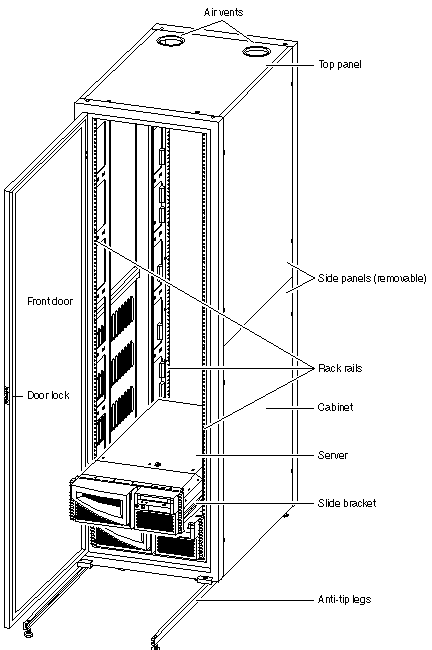
\includegraphics[height=0.6\paperheight]{cabinet}
\end{center}

\subsubsection{Rack airflow direction}

\begin{center}
  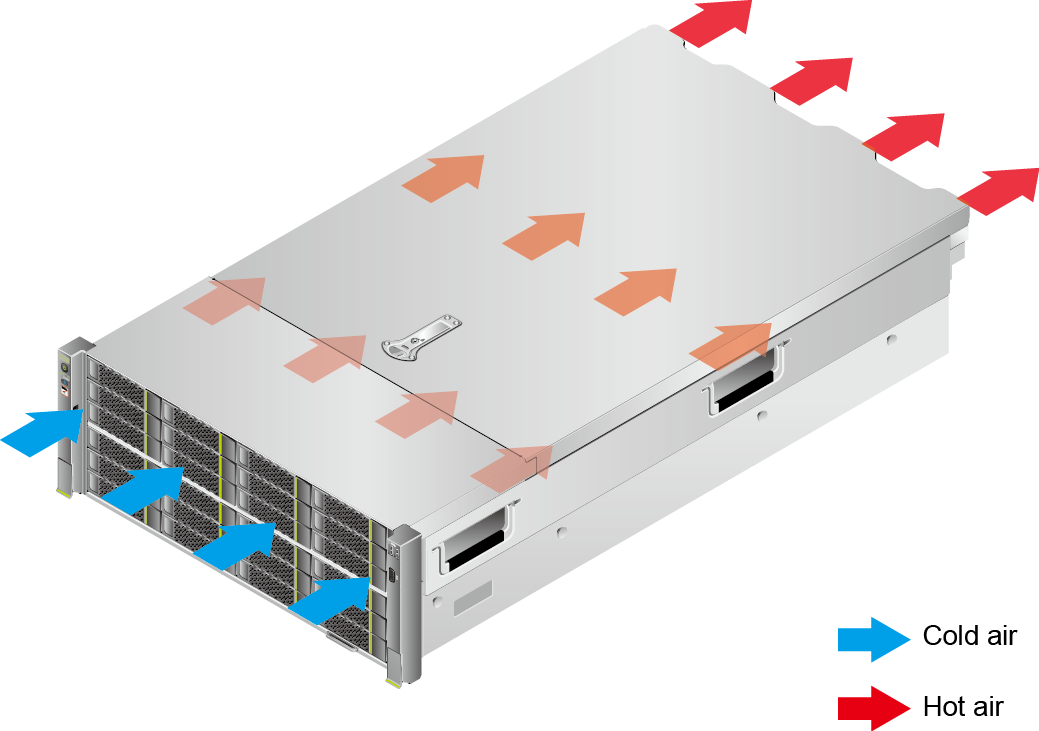
\includegraphics[width=0.6\linewidth]{server_airflow_huawei}
\end{center}

\section{Power}

Servers and other IT equipment require mains power to operate.

Interruptions or disturbances in the power supply may affect service availability.

\subsection{Uninterruptible Power Supplies}

\textbf{Uninterruptible Power Supply (UPS) equipment ensures that a host is protected from short-term power outages and glitches in the power supply.}

\begin{center}
\includegraphics[width=0.9\linewidth]{ups}
\end{center}

\begin{description}
\item[Normal conditions] can correct minor power glitches
\item[Short outages] can power hosts from battery
\item[Longer outages] can signal hosts to safely shut down
\end{description}

\subsection{Generators}

\textbf{Generators can be used to extend run-time during power loss.}

\begin{center}
\includegraphics[width=0.7\linewidth]{generator}
\end{center}

\subsection{Redundant power paths}

\begin{center}
\includegraphics[width=0.6\linewidth]{redundant_power}
\end{center}


\section{Connectivity}

\textbf{Host requires connection to a network}

\begin{greenbox}{Options}
  \begin{itemize}
  \item Directly on the internet with a Public IP address.
  \item On an internal network with a private IP address.
  \item Internal network but has a NAT public IP address.
  \item Internal network with a VPN for remote users.
  \end{itemize}
\end{greenbox}

\begin{bluebox}{Meet-Me Room (MMR)}
  Co-location data centres usually have a Meet-Me Room (MMR):
  \begin{itemize}
  \item Internet Providers termination here
  \item Cross-connected to customer rack
  \end{itemize}
\end{bluebox}

\section{Cooling}

Heat removal is necessary for all data centre environments.

\begin{bluebox}{Where does the heat come from?}
  \begin{itemize}
  \item Almost all the electrical power input to IT equipment is converted to heat.
\item Without any means to remove heat, the temperature in the closed space will rise quickly.
  \end{itemize}
\end{bluebox}


\subsection{Temperature}
\label{sec:temperature}

\textbf{Temperature numerically quantifies how hot something is}

The most common conversion is to/from Fahrenheit.
\begin{align}
  T_C & = \frac{T_F-32}{1.8} \label{eq:f-to-c} \\
  \Rightarrow  T_F & = T_C \times 1.8 + 32 \label{eq:c-to-f}
\end{align}

The Kelvin scale is rarely encountered in applied settings but is directly related to the Celsius scale:
\begin{align}
  T_C & = T_K - 273 \label{eq:k-to-c} \\
  T_K & = T_C + 273 \label{eq:c-to-k} 
\end{align}


\begin{table}[htbp]
  \centering
  \includegraphics[width=0.4\linewidth]{temp_scales_ahrens}
  \caption{Temperature Scales (Ahrens 1994)}
  \label{tab:temp-scales}
\end{table}

\subsection{Thermal envelope}
\label{sec:thermal-envelope}

\textbf{Equipment and humans can only tolerate a certain range of temperatures, or thermal envelope.}

\begin{redbox}{Outside thermal envelope}
  \begin{description}
  \item[CPU throttling:] reducing speed to reduce heat output
  \item[Thermal shutdown] causing host to become unavailable
  \item[Reduced lifespan] due to thermal stress
  \end{description}
\end{redbox}

American Society of Heating, Refrigeration and Air conditioning Engineers (ASHRAE) recommended thermal envelope is between 18 and 27 degrees.


\subsection{Cooling methods}

In order to keep the temperature and relative humidity within permitted limits, we must rely on some method of cooling.

\begin{bluebox}{Options}
\begin{description}
\item[Conduction] uses the room's surfaces to remove heat to the surrounding building.
\item[Passive ventilation] involves vents placed appropriately within the room to permit hot air to flow naturally out, to be replaced by cooler incoming air.
\item[Fan-assist ventilation] works similarly to passive ventilation, but the air movement is assisted by a fan.
\item[Dedicated cooling] is where the room air is not ventilated, but instead heat is removed from it. 
\end{description}
\end{bluebox}

\autoimage{cooling_method_guide}{Cooling methods (APC)}{cooling-methods}


\subsection{Fan-assisted ventilation}

Fans can be used on in smaller data centre environments to keep the temperature under control by exchanging the air with the ambient / outside environment.

\begin{itemize}
\item Fans can be thermostatically controlled.
\item Can be powered from a UPS to ensure the fans run even when mains power fails. 
\end{itemize}

\begin{redbox}{Limitations}
  \begin{itemize}
  \item In practical terms, anything more than a simple closet with a few devices will need refrigerated cooling.
  \item Conduction, passive ventilation and fan-assisted cooling schemes are ultimately limited by the outdoor temperature.
  \item Consider trying to keep a room at 22C when the outdoor temperature is 34C!
  \end{itemize}
\end{redbox}

\newpage

\begin{center}
  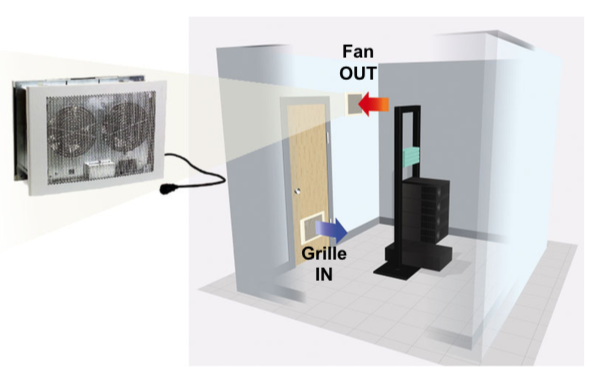
\includegraphics[height=0.7\paperheight]{fan_assisted_ventilation}
\end{center}



\subsection{Refrigeration cycle}

\begin{bluebox}{Refrigeration cycle stages}
  \begin{small}
\begin{enumerate}
\item Cold liquid refrigerant in the \textbf{evaporator} is warmed by air passing over it, and boils at roughly \SI{7.8}{\degreeCelsius}. The air passing over the evaporator gives up some of its heat energy. It leaves at a cooler temperature than it entered at.
\item The \textbf{compressor} increases the pressure of the gaseous refrigerant, greatly increasing its temperature to over \SI{50}{\degreeCelsius}.  In doing so, it also acts as a pump for the refrigerant around the loop, which is carrying the heat energy to reject.
\item Hot gaseous refrigerant enters the \textbf{condenser} coil, across which is circulated outside air. As the refrigerant is hotter than the outside air, it gives up its heat to the outside air.  The air passing over the condenser receives heat energy from the hot refrigerant, leaving at a warmer temperature than it entered at. The refrigerant is cooled below its boiling point and changes phase to a liquid.  It will still be quite hot to the touch!
\item The warm liquid flows through the \textbf{expansion valve}, which limits the flow of refrigerant such that it is boiled off in the evaporator. When the refrigerant emerges from the expansion valve, it expands since the flow is limited, and is ready for another cycle in the evaporator. 
\end{enumerate}
\end{small}
\end{bluebox}

\autoimage{refrigeration_cycle}{Refrigeration cycle}{refrigeration-cycle}


\subsection{Computer Room Air Conditioners}

\begin{itemize}
\item Warm \textbf{return air} enters the CRAC via an opening on the top of the unit.
  Sometimes the return air is ducted to the unit from above the ceiling.
\item Cold \textbf{supply air} leaves the CRAC via an opening in the bottom:
  \begin{itemize}
  \item If there is a raised floor, the cold air is blown out the bottom of the unit under the raised floor.
    It flows under the raised floor and exits through perforated tiles.
  \item In the case of a solid floor, the cold air normally leaves via a large grille on the bottom of the unit.
  \end{itemize}
\end{itemize}
Other configurations include upflow (reverse of the above, but only on a solid floor), horizontal and other configurations.
Cooling units are sometimes located in other areas and ducted to the data centre environment.

\autoimage{crac_photo}{Computer Room Air Conditioner}{crac-photo}

\subsubsection{Airflow}

For the cooling system to work properly, we \textbf{must use a hot aisle / cold aisle arrangement}.
Where a raised floor is used, the perforated tiles must be in the cold aisle, and not in the hot aisle.

\autoimage{cooling_airflow}{Airflow from Downflow CRAC through raised floor}{cooling-airflow}

\subsubsection{Self-contained air-cooled DX}
\label{sec:self-contained-air-cooled-dx}

Self-contained units have all refrigeration components within the CRAC's casing, \autoref{fig:crac-dx-self-contained}.

\begin{figure*}[hptb]
  \centering
  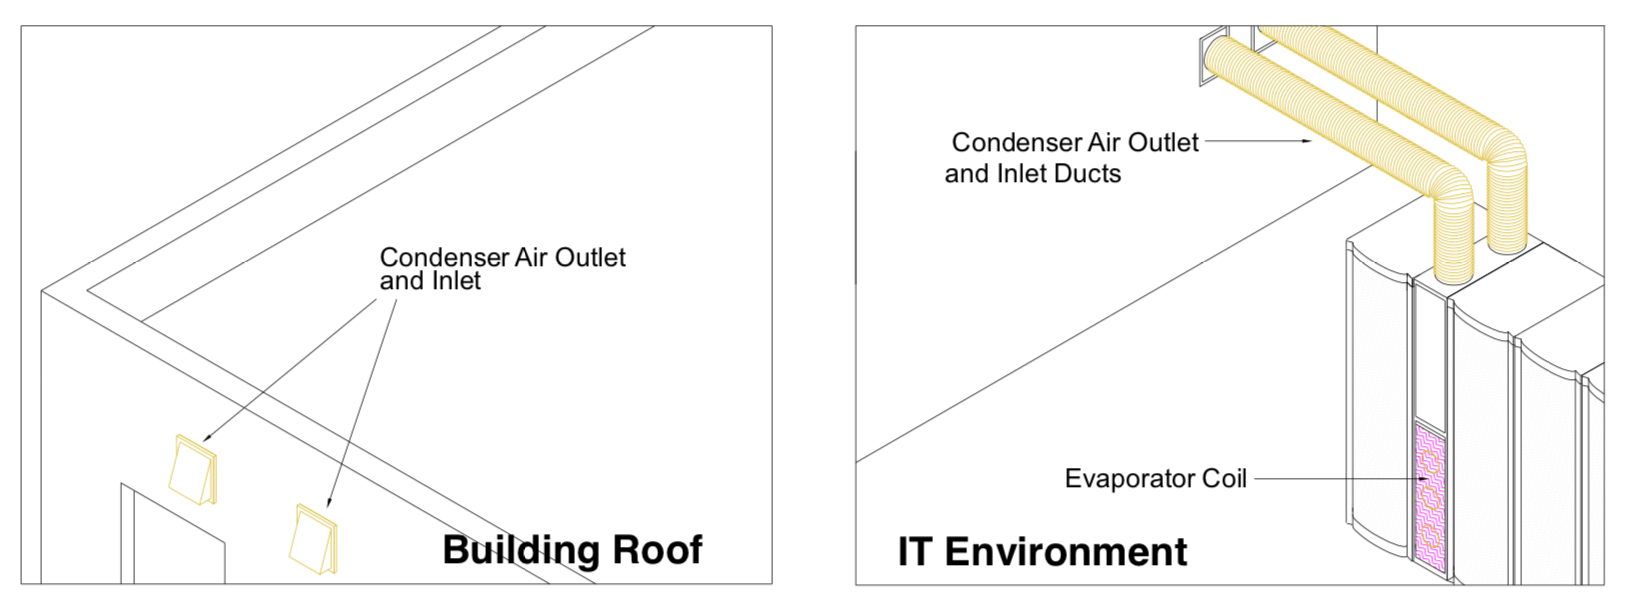
\includegraphics[width=1.0\linewidth]{crac_self_contained_schematic}
  \caption{DX self-contained CRAC (APC)}
  \label{fig:crac-dx-self-contained}
\end{figure*}

The condenser supply and exhaust are ducted from the outdoors.

\begin{greenbox}{Usage}
  \begin{itemize}
  \item Limited in cooling capacity to approx \SI{15}{\kilo\watt} due to unit size and ducting
  \item Often seen in small on-site server rooms.
  \end{itemize}
\end{greenbox}




\subsubsection{Air-Cooled DX}
\label{sec:air-cooled-dx}

Direct expansion, often abbreviated DX, cooling systems house the evaporator, compressor and expansion valve within the CRAC unit.
The condenser is sited externally, with wiring and refrigerant connections from the CRAC unit, \autoref{fig:crac-dx-air}.

\begin{figure*}[hptb]
  \centering
  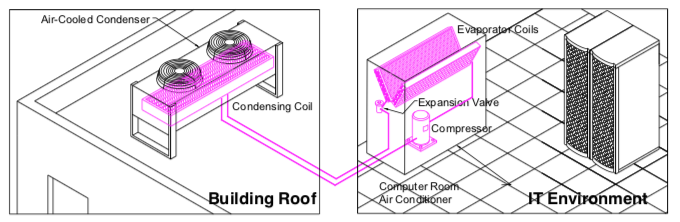
\includegraphics[width=1.0\linewidth]{crac_dx_air_schematic}
  \caption{DX air-cooled CRAC with condenser (APC)}
  \label{fig:crac-dx-air}
\end{figure*}

\begin{greenbox}{Usage}
  \begin{itemize}
  \item Candidate for \SIrange{7}{200}{\kilo\watt}.
  \item Multiple units often used for larger capacities and to provide redundancy (see later).
  \end{itemize}
\end{greenbox}

\autoimage{condenser_photo}{Condenser}{condenser-photo}


\subsubsection{Chilled water cooling systems}

\textbf{Chilled water cooling systems involve the supply of chilled water to Computer Room Air Handlers (CRAH) in the data centre environment.}

The chilled water is produced in a separate \textit{chiller}.

The chiller rejects heat from the chilled water loop to the atmosphere in similar ways to DX CRACs:

Normally large number of CRAHs served by a small number of chillers and cooling towers.

Chilled water systems also can incorporate large buffer tanks for load balancing, energy price optimisation and to provide \textit{ride through} in case of power failure.


In a multi-tenant building, the landlord will often supply chilled water as a metered chargeable service to tenants.

\begin{figure}[htbp]
  \centering
  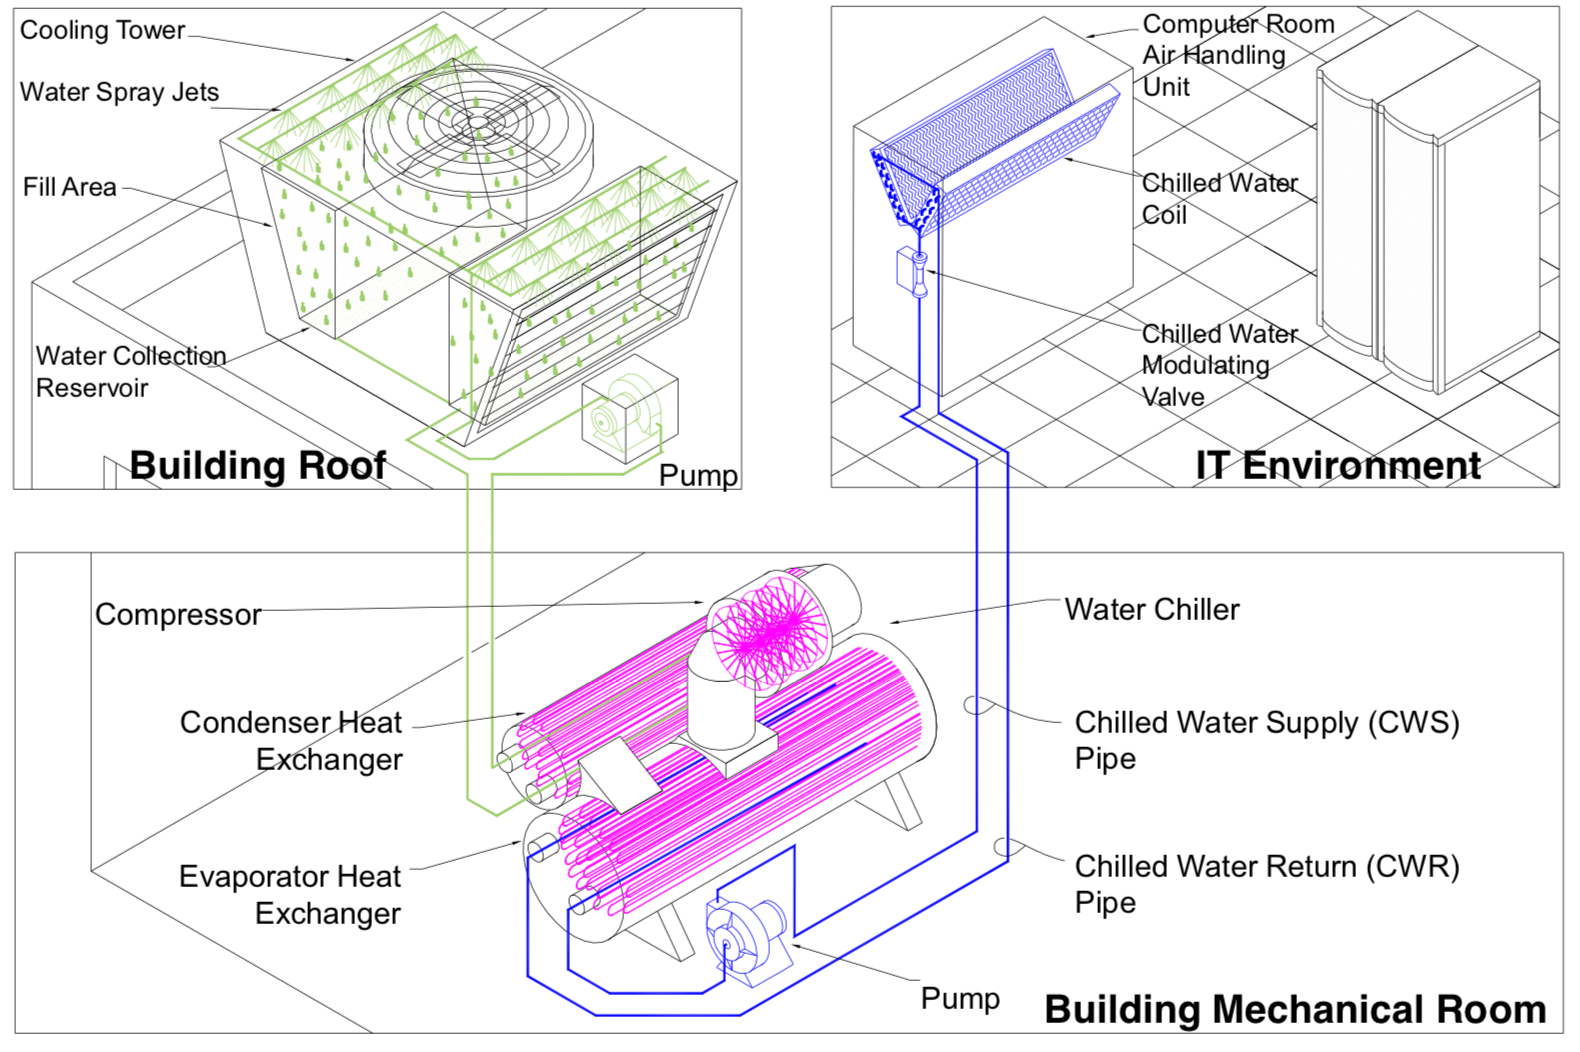
\includegraphics[width=0.7\linewidth]{chilled_water_system_water_cooled}
  \caption{Chilled water system}
  \label{fig:chilled-water-system-water-cooled}
\end{figure}



\end{document}
